\begin{frame}
  {\texttt{\$ who}}

  \begin{columns}
    \begin{column}{0.48\textwidth}
      {\texttt{@f0rki}}
      \begin{itemize}
        \item f0rki@hack.more.systems 
        \item InfoSec Student
        \item CTF Player since 2010
      \end{itemize}
    \end{column}

    \begin{column}{0.48\textwidth}
      \texttt{@stefan2904}
      \begin{itemize}
        \item stefan@hack.more.systems
        \item InfoSec Student
        \item CTF Player since 2014
      \end{itemize}
    \end{column}
  \end{columns}

\end{frame}


\begin{frame}{stuff we are gonna be talking about \ldots}
    \tableofcontents
\end{frame}


\section{Introduction to CTFs}

\begin{frame}[fragile]
  {CTF: Capture The Flag}

  \begin{itemize}
    \item Collaborative hacking competitions
    \begin{itemize}
    	\item Teams vs. Teams
    \end{itemize}
    \item The goal is to capture flags
      %\begin{itemize}
        %\item Like \\
        %  \verb+9447{ffmpeg_m0re_like_ffRCE_amirite}+ \\
        %  or \\
        %  \verb+FAUST_VnSn2AwDAd1XxAAAAACjEEhYAjVLomA1+
        %\item More flags \verb+==+ more points
      %\end{itemize}
    \item Hack stuff and get flags
  \end{itemize}
\end{frame}



\begin{frame}[fragile]{}
	 \begin{center}
	 	\Huge\verb+CTF{THIS_IS_A_FLAG}+
	 \end{center}
\end{frame}

\begin{frame}
  {CTF Type: Jeopardy}

  \begin{center}
    %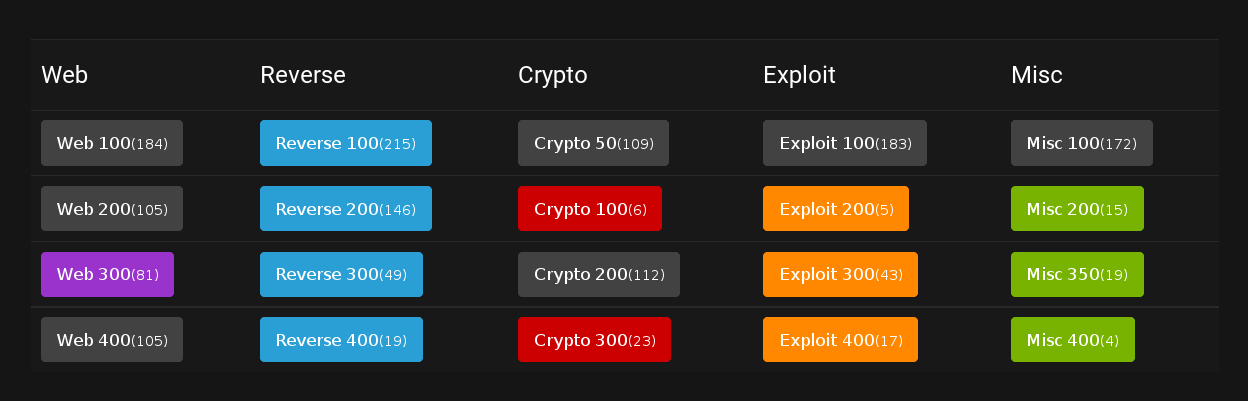
\includegraphics[width=\textwidth]{./images/dctf-challenges.png}
    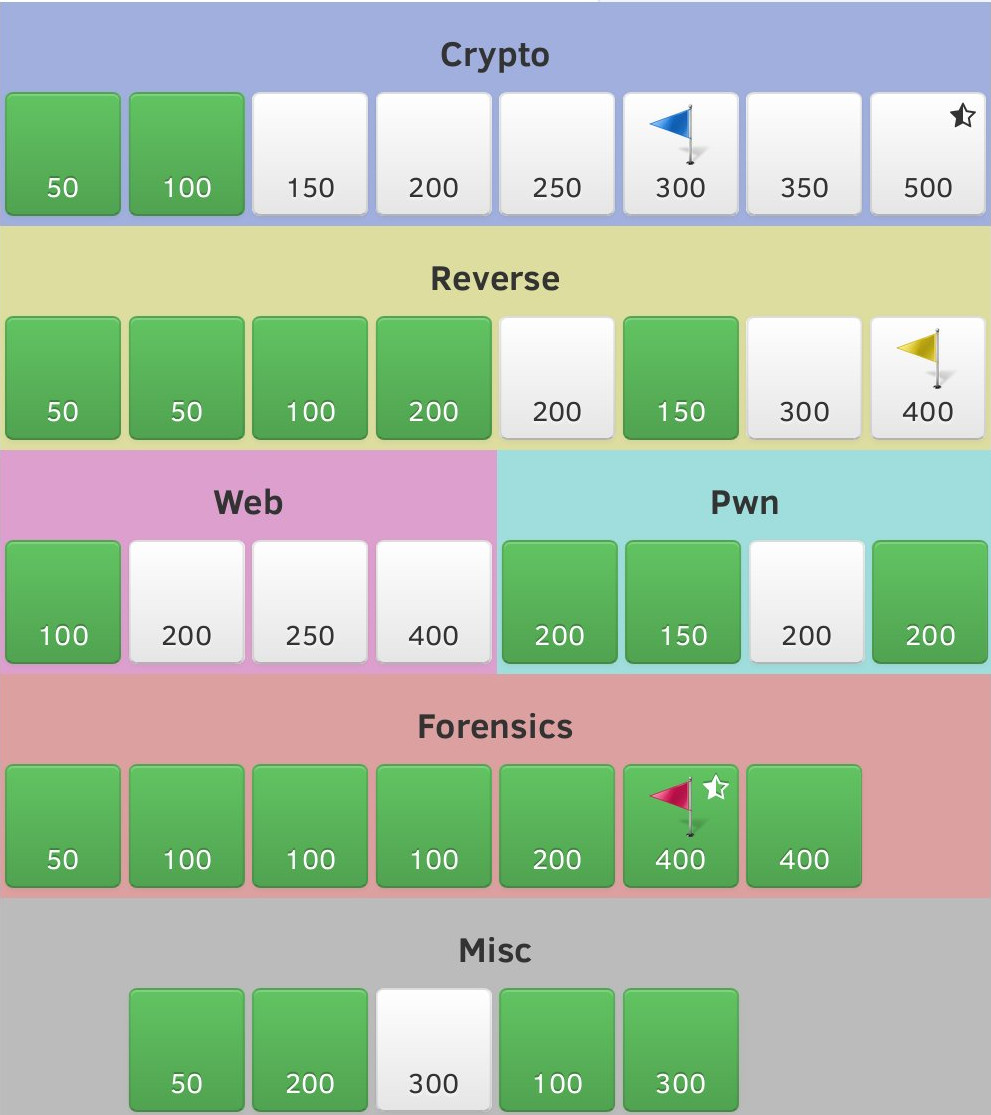
\includegraphics[height=0.8\textheight]{./images/sharifctf-challenges.jpg}
  \end{center}
\end{frame}

\begin{frame}
  {CTF Type: Attack-Defense}

  \begin{figure}[h]
    \centering
    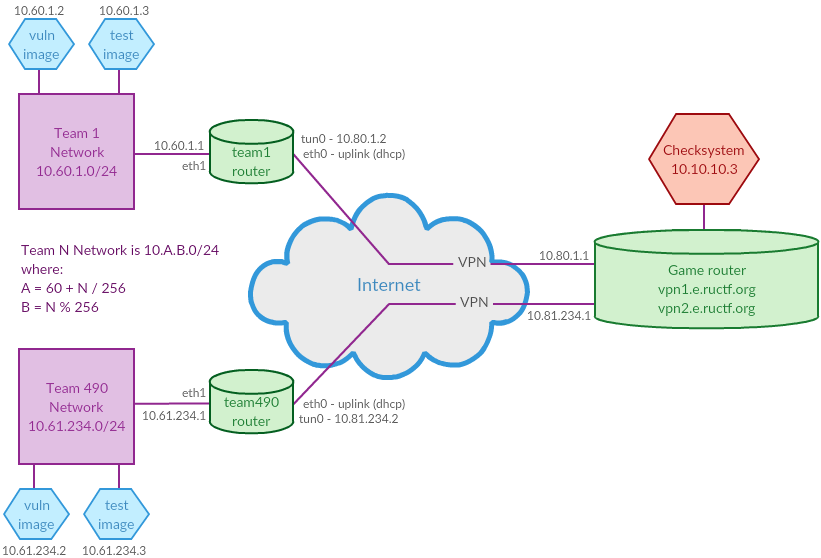
\includegraphics[width=0.9\textwidth]{./images/ructf-network.png}
    \caption{RUCTFe 2015 Network Schema (source:
      \href{https://ructf.org/e/2015/network.html}{RUCTF org}) }
  \end{figure}
\end{frame}
\begin{frame}
  {CTF Type: Attack-Defense}

  \begin{center}
    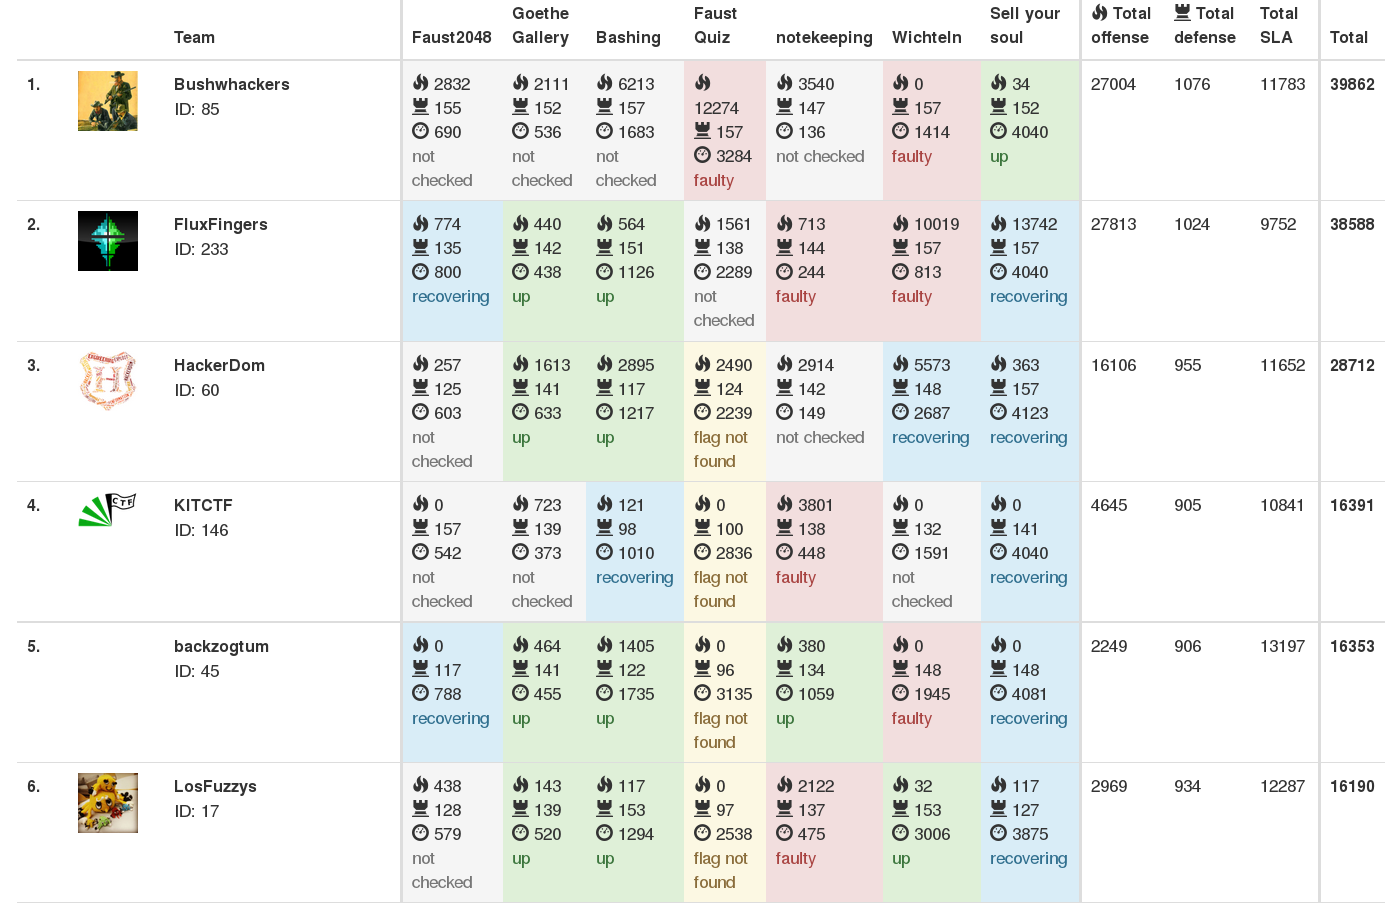
\includegraphics[width=\textwidth]{./images/faustctf-scoreboard.png}
  \end{center}

\end{frame}


\begin{frame}
  {Why CTFs?}

  \begin{itemize}
    \item \textbf{It's fun!}
    \item Gain experience in InfoSec
    \item Challenges modeled after real-world problems
      \begin{itemize}
        \item Sometimes real-world bugs modeled after CTF bugs?
      \end{itemize}
  \end{itemize}
\end{frame}

\section{LosFuzzys}

\begin{frame}[allowframebreaks]
  {\texttt{LosFuzzys}: A CTF Team in Graz}
  {We Like Bugs!}

  \begin{figure}[H]
    \centering
    \includegraphics[height=0.7\textheight]{images/zippy/zippy_family2.jpg}
  \end{figure}

  \framebreak

  \begin{itemize}
    \item \url{https://hack.more.systems}
      \\ twitter: \href{https://twitter.com/LosFuzzys}{@LosFuzzys}
    \item A group of people interested in information security
    \item Primarily CS/SW/ICE Students from TUGraz
      \begin{itemize}
        \item But we welcome anyone interested and motivated :)
        \item and maybe even you ;)
      \end{itemize}
    \item Irregular Meet-ups
  \end{itemize}
\end{frame}

\begin{frame}
	{Where to start?}
	
	\begin{itemize}
		\item Talk to us! :-)
	\end{itemize}
	
	\begin{itemize}
		\item Read writeups!
		\begin{itemize}
			\item Repo: \href{https://github.com/ctfs}{github.com/ctfs}
			\item Ours: \href{https://hack.more.systems/writeups}{hack.more.systems/writeups}
		\end{itemize}
	\end{itemize}
	
\end{frame}

\section{CTF Toolbox}

\begin{frame}
  {CTF Hackers Toolbox}

  \begin{itemize}
    \item Great diversity of challenges
    \item Some things turn up frequently
    \item Knowledge of technology necessary
    \item Experience helps a lot
  \end{itemize}

  \begin{itemize}
    \item Using the right tools is essential
      \begin{itemize}
        \item assuming you know how to use them\ldots
      \end{itemize}
  \end{itemize}

\end{frame}

\begin{frame}
  {Scripting is your best Friend}

  \begin{itemize}
    \item Python, Ruby, Bash etc.
    \item Be comfortable in one of those
  \end{itemize}

  \begin{center}
    
\includegraphics[height=0.5\textheight]{images/automatealltheexploits.jpg}
  \end{center}
\end{frame}


\begin{frame}
  {Command-Line-Fu is very helpful}

  \begin{itemize}
    \item Network stuff -- \texttt{nc, socat, dig, nmap}
    \item Query json files -- \texttt{jq}
    \item HTTP -- \texttt{curl}
  \end{itemize}

  \begin{itemize}
    \item Chain together to get your results!
  \end{itemize}
\end{frame}

% python requests - automated browsing

\begin{frame}[fragile]
  {Automated Browsing -- python-requests}

  \begin{lstlisting}[language=python]
import requests
s = requests.session()
URL = 'http://ctf.example.com'
r = s.post(URL + '/login',
           data={'user': 'fuzzy', 'pass': '1234'})
# session cookie automagically used here
print s.get(URL + '/vuln', params={'x': 'or/**/1=1--x'}).text
# GET 'http://ctf.example.com/vuln?x=or/**/1=1--x
  \end{lstlisting}
\end{frame}

% pwntools - implement parts of line-based network protocols

\begin{frame}[fragile]
  {dirty networking -- pwntools/binjitsu}

% TODO: send email or something
  \begin{lstlisting}[language=python]
from pwn import *
r = remote('ctf.example.com', 1337)
r.recvline()  # ignore
r.sendline('HELO %p%p%p%p')
r.recvuntil('250 Hello')
data = r.recv(2 + 4 * 2)
r.recvline()
  \end{lstlisting}
\end{frame}

% pwntools - build exploits and pwn binaries

% radare2 - hex editor and disassembler

% gdb - pretty horrible
%peda
%https://github.com/cyrus-and/gdb-dashboard
%voltron

% retdec decompiler

% pen & paper - never underestimate

% sagemath - crypto all the things

% apktool - disassemble and patch android apps



\begin{frame}
  {Learn to Improvise}

  \begin{itemize}
    \item Premature optimization* is the root of all evil!
      \begin{itemize}
        \item * also commenting code
        \item * also clean code
      \end{itemize}
    \item (only true for attack \&\&  \emph{during} CTFs!)
    \item If it works, \ldots it works!
    \item Code-reuse between different CTFs
  \end{itemize}

\end{frame}

\begin{frame}
	\begin{center}
		\huge A fool with a tool is still a fool!
	\end{center}
\end{frame}

\begin{frame}
  {}
\end{frame}
